\chapter{Denoising using the Mean of Noisy Instances (MNI)}
%{{{

\section{The central limit theorem}
\label{sec:CLT}
%{{{

The \gls{CLT} states that when a set of independent \glspl{SRV} (see
Section~\ref{sec:DSRV}) are added together, the \gls{SRV} resulting of their normalized sum tends
toward a normal (Gaussian) distribution, even if the original
variables themselves are not normally distributed. Let
$\mathbf{n}=\{\mathbf{n}^{(i)}\}_{i=0}^{N-1}$ such set of independent and
identically distributed (i.i.d.) \glspl{SRV}, then the \gls{CLT} states that the mean signal
\begin{equation}
  \overline{n} = \frac{1}{N}\sum_{i=0}^{N-1}\mathbf{n}^{(i)}\sim\mathcal{N}(\mu,\frac{\sigma}{N}),
\end{equation}
where
\begin{equation}
  \mathbb{E}(\mathbf{n}^{(i)})=\mu\quad\forall i,
\end{equation}
and
\begin{equation}
  \mathbb{V}(\mathbf{n}^{(i)})=\sigma\quad\forall i.
\end{equation}
Notice that
\begin{equation}
  \lim_{N\rightarrow\infty}\mathbb{V}(\overline{\mathbf{n}}) = 0.
\end{equation}

%}}}

\section{\glsentryfull{GAT}}
The \acrshort{GAT} \cite{foi2008practical,makitalo2012optimal} is a
\gls{VST} that can be applied to \gls{MPG} noise (see
Section~\ref{sec:MPG}) to make it approximately Gaussian with
(approximately) constant variance of $1$, so we can apply standard
Gaussian denoisers (e.g., \gls{BM3D}, \gls{DnCNN}, wavelet shrinkage,
etc.). It consists of converting the noisy samples using the
expression
\begin{equation}
  y = \text{GAT}(\hat{\mathbf{s}}_i)=\frac{2}{\gamma}\sqrt{\gamma\hat{\mathbf{s}}_i+\frac{3}{8}\gamma^2+\sigma^2},
\end{equation}
where now
\begin{equation}
  y\sim\mathcal{N}(\mu',\approx 1).
\end{equation}
$\gamma$ is an empirical value that controls the gain of the transform.

Notice that the \gls{GAT} is not a linear transform and that the mean is
not preserved, in neither of the directions of the transform. This
basically implies that to recover the original mean by simply
inversing the forward expression. For this reason, in
\cite{makitalo2012optimal} (among others) the following approximation
can be used only if we deal with positive transformed values and $\mu=0$:
\begin{equation}
  \hat{\mathbf{s}}_i \approx \frac{1}{4}y^2-\frac{1}{4}\left(1+\frac{8\sigma^2}{y^2} + \frac{1}{32}\left(\frac{i+\frac{8\sigma^2}{y^2}}{y^2}\right)\right).
\end{equation}

\section{\glsentryfull{MNI}}
Under a high enough number of noisy instancces, the \gls{CLT} allows
us to take into consideration only the \gls{AWG} noise case (see
Section~\ref{sec:AWG}) when we perform denoising throught computing
the mean of those noisy instances. Let
\begin{equation}
  \hat{\mathbf{s}}^{(i)} = \mathbf{s} + \mathbf{n}^{(i)},
  \label{eq:noisy_instances}
\end{equation}
the generation of the $i$-th noisy instance of the
signal $\mathbf{s}$. Assuming that
\begin{equation}
  \mathbb{E}(\mathbf{n})=\mathbf{0},
\end{equation}
where $\mathbf{n}=\{\mathbf{n}^{(i)}\}_{i=0}^{N-1}$ is the set of
random signals, and taking expectations in
Eq.~\ref{eq:noisy_instances}, we get
\begin{equation}
  \mathbb{E}(\hat{\mathbf{s}}) = \mathbb{E}(\mathbf{s}) + \mathbb{E}(\mathbf{n}) = \mathbf{s},
  \label{eq:MNI}
\end{equation}
where
$\hat{\mathbf{s}}=\{\hat{\mathbf{s}}^{(i)}\}_{i=0}^{N-1}$. Notice,
however, that Eq.~\ref{eq:MNI} is only true when
$N\rightarrow\infty$. In practice, where $N$ is finite, we only get an
approximation $\tilde{\mathbf{s}}^{[N]}$, where $N$ is the number of
averaged signals.

\section{Experiments}
%{{{

This section is basically an experimental verification of the
efficiency of the \gls{CLT} (see
Section~\ref{sec:CLT}). Figure~\ref{fig:MNI_0MMPG} shows an example of
how \gls{MNI} increases the quality using images with \gls{MPG} noise.
  
\begin{figure}
  \centering
  \resizebox{1.0\textwidth}{!}{
    \renewcommand{\arraystretch}{0.0} % Adjust row spacing in the table
    \setlength{\tabcolsep}{0ex}      % Adjust column spacing in the table    
    \begin{tabular}{cc}
      \href{https://nbviewer.org/github/vicente-gonzalez-ruiz/denoising/blob/main/notebooks/barb.ipynb\#barb}{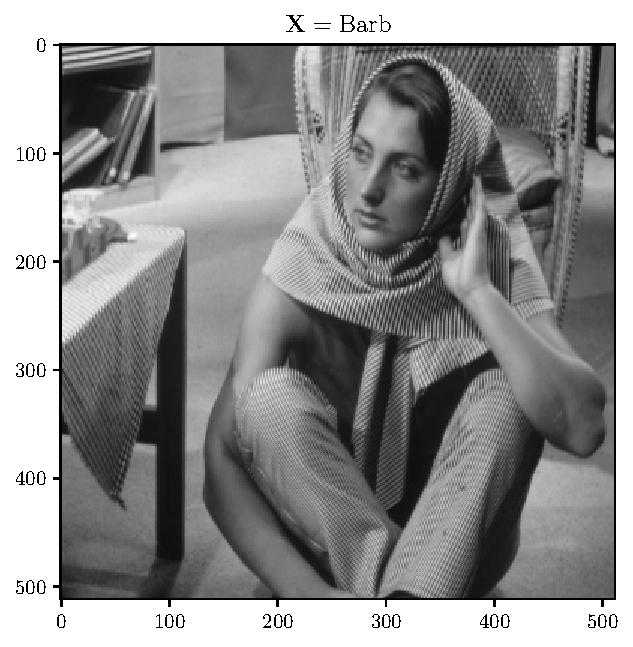
\includegraphics{barb.pdf}} & \href{https://nbviewer.org/github/vicente-gonzalez-ruiz/denoising/blob/main/notebooks/barb_0MMPG.ipynb\#barb_0MMPG}{\includegraphics{barb_0MMPG.pdf}} \\
      \href{https://nbviewer.org/github/vicente-gonzalez-ruiz/denoising/blob/main/notebooks/barb_averaging.ipynb\#barb_averaging}{\includegraphics{barb_averaging.pdf}} & \href{https://nbviewer.org/github/vicente-gonzalez-ruiz/denoising/blob/main/notebooks/barb_averaging_PSNR.ipynb\#barb_averaging_PSNR}{\includegraphics{barb_averaging_PSNR.pdf}}
    \end{tabular}
  }
  \caption{Increase of the SNR as a function of the number of noisy
    instances used in MNI. The clean image is shown on the top-left,
    and a noisy instance on the top-right. On the bottom-left, the
    denoised NMI image, and on the bottom-right the progression of the
    SNR as a function of $I$ and the level of
    noise.\label{fig:MNI_0MMPG}}
\end{figure}

\begin{comment}
%{{{

Fig.~\ref{fig:0MAUN} shows an
example of how zero-mean uniform noise is cancelled by averaging.
  
  \begin{figure}
    \centering
    \resizebox{1.0\textwidth}{!}{
      \renewcommand{\arraystretch}{0.0} % Adjust row spacing in the table
      \setlength{\tabcolsep}{0ex}      % Adjust column spacing in the table    
      \begin{tabular}{cc}
        \href{https://nbviewer.org/github/vicente-gonzalez-ruiz/denoising/blob/main/figs/averaging_denoising.ipynb\#Display-Barb}{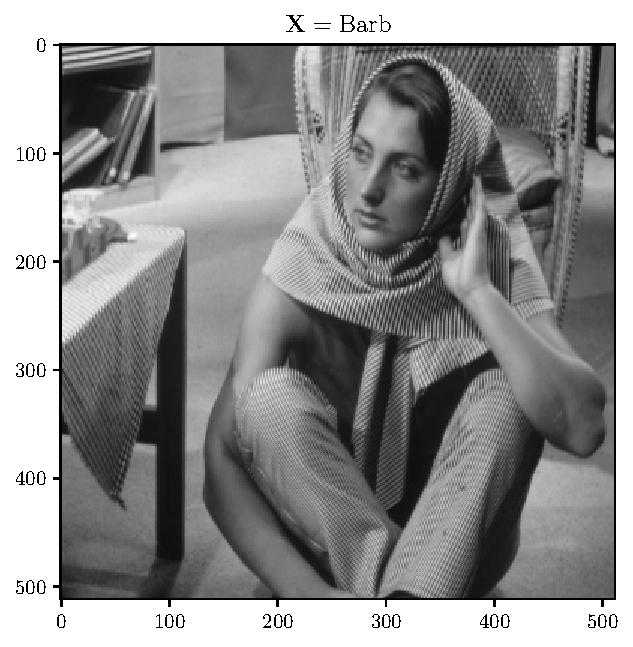
\includegraphics{barb}} & \href{https://nbviewer.org/github/vicente-gonzalez-ruiz/denoising/blob/main/figs/averaging_denoising.ipynb\#0MAUN_barb}{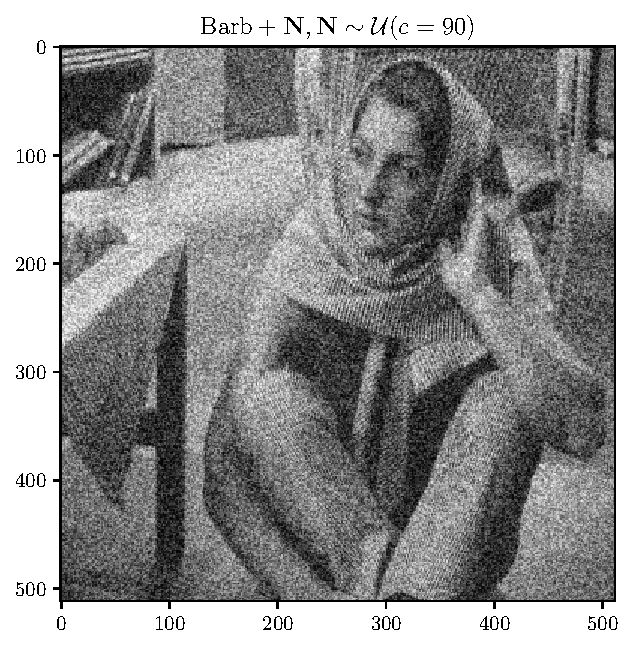
\includegraphics{0MAUN_barb}} \\
        \href{https://nbviewer.org/github/vicente-gonzalez-ruiz/denoising/blob/main/figs/averaging_denoising.ipynb\#denoised_0MAUN_barb}{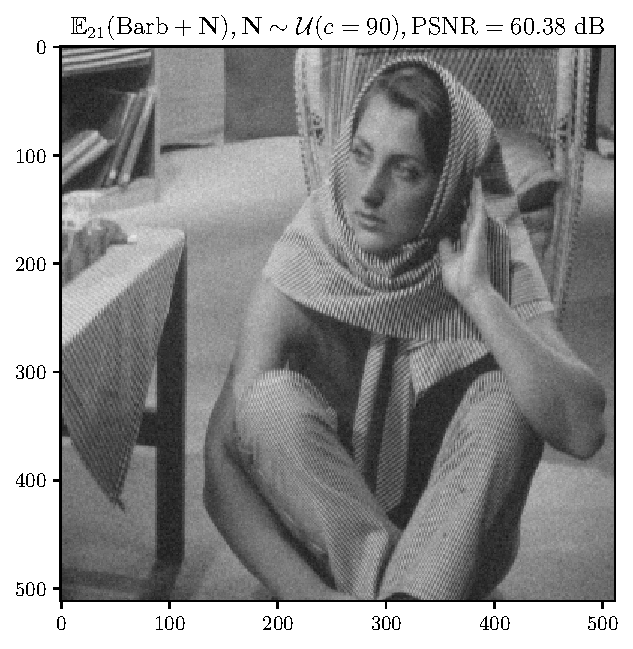
\includegraphics{denoised_0MAUN_barb}} & \href{https://nbviewer.org/github/vicente-gonzalez-ruiz/denoising/blob/main/figs/averaging_denoising.ipynb\#PSNR_0MAUN_barb}{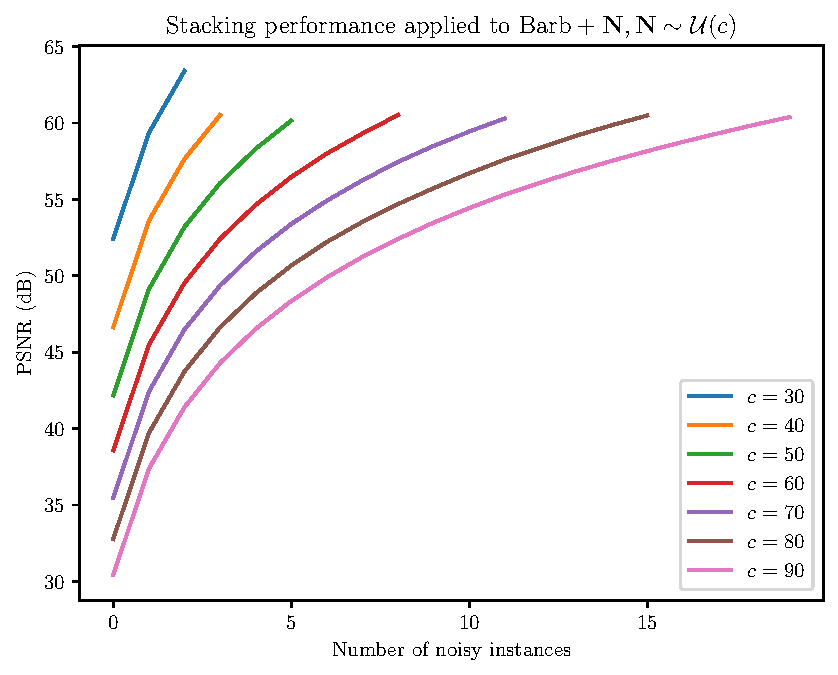
\includegraphics{PSNR_0MAUN_barb}}
      \end{tabular}
    }
    \caption{Effect of zero-mean additive uniform noise in an image
      and how averaging can be used to reduced by averaging. The clean
      image of Barb is shown on the top left, and a noisy version on
      the top right. On to bottom, the left image shows a denoised
      version after averaging and the right graph shows the performance
      of the averaging process for different levels of
      noise.\label{fig:0MAUN}}
  \end{figure}

 Fig.~\ref{fig:0MAGN} shows an
  example of how zero-mean Gaussian noise is cancelled by averaging.

  \begin{figure}
    \centering
    \resizebox{1.0\textwidth}{!}{
      \renewcommand{\arraystretch}{0.0} % Adjust row spacing in the table
      \setlength{\tabcolsep}{0ex}      % Adjust column spacing in the table    
      \begin{tabular}{cc}
        \href{https://nbviewer.org/github/vicente-gonzalez-ruiz/denoising/blob/main/figs/averaging_denoising.ipynb\#barb}{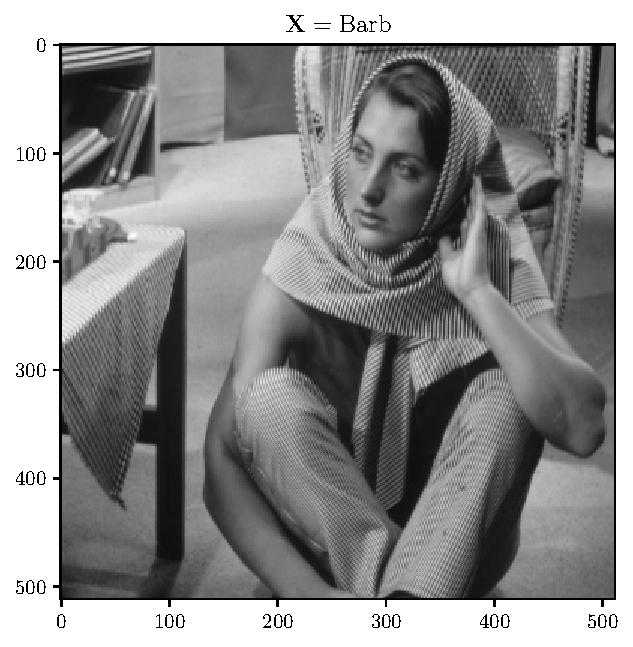
\includegraphics{barb}} & \href{https://nbviewer.org/github/vicente-gonzalez-ruiz/denoising/blob/main/figs/averaging_denoising.ipynb\#0MAGN_barb}{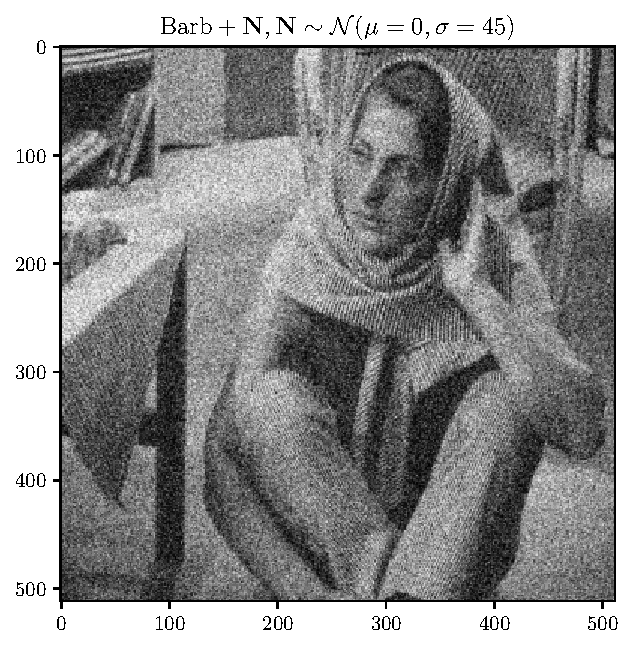
\includegraphics{0MAGN_barb}} \\
        \href{https://nbviewer.org/github/vicente-gonzalez-ruiz/denoising/blob/main/figs/averaging_denoising.ipynb\#denoised_0MAGN_barb}{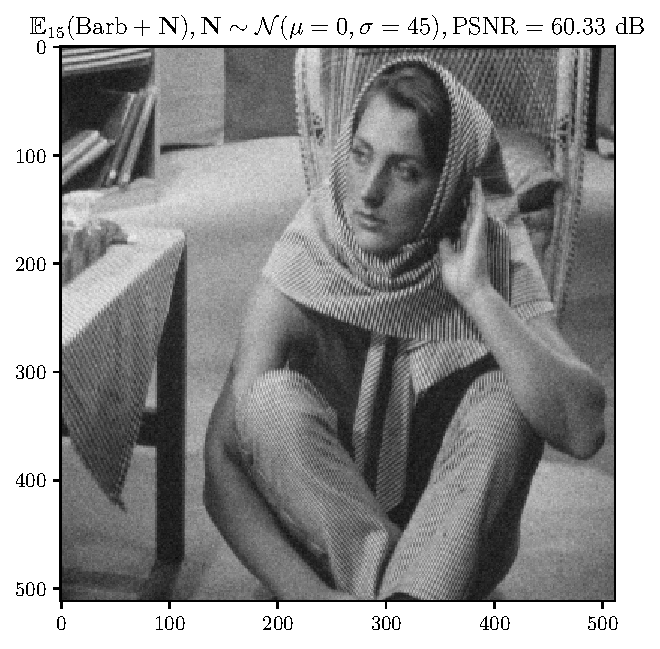
\includegraphics{denoised_0MAGN_barb}} & \href{https://nbviewer.org/github/vicente-gonzalez-ruiz/denoising/blob/main/figs/averaging_denoising.ipynb\#PSNR_0MAGN_barb}{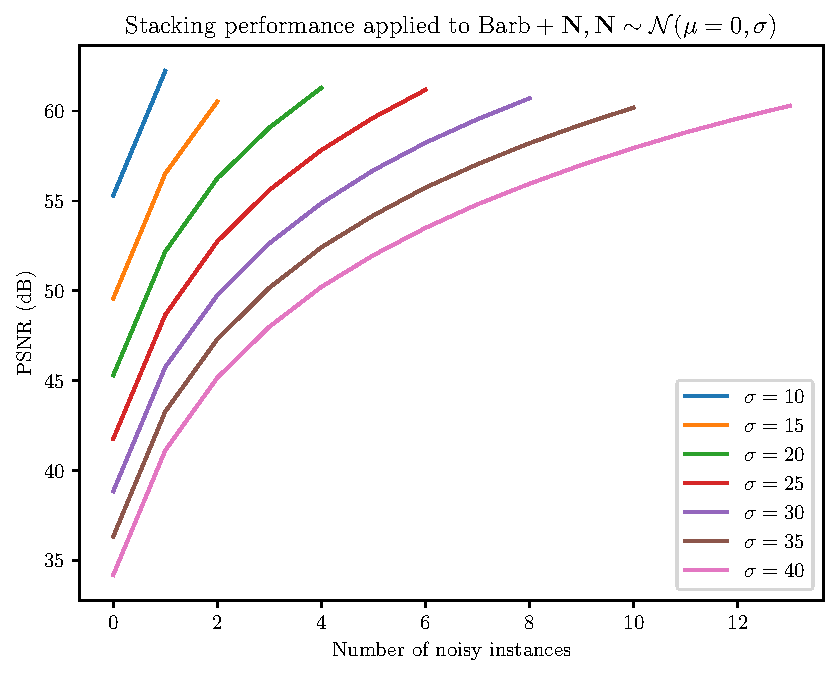
\includegraphics{PSNR_0MAGN_barb}}
      \end{tabular}
    }
    \caption{Effect of zero-mean additive Gaussian noise in an image
      and how averaging can be used to reduced by averaging. The clean
      image of Barb is shown on the top left, and a noisy version on
      the top right. On to bottom, the left image shows a denoised
      version after averaging and the right graph shows the performance
      of the averaging process for different levels of
      noise.\label{fig:0MAGN}}
  \end{figure}

  Fig.~\ref{fig:0MMGN} shows an example of
  how zero-mean Gaussian noise is cancelled by averaging.

  \begin{figure}
    \centering
    \resizebox{1.0\textwidth}{!}{
      \renewcommand{\arraystretch}{0.0} % Adjust row spacing in the table
      \setlength{\tabcolsep}{0ex}      % Adjust column spacing in the table    
      \begin{tabular}{cc}
        \href{https://nbviewer.org/github/vicente-gonzalez-ruiz/denoising/blob/main/figs/averaging_denoising.ipynb\#barb}{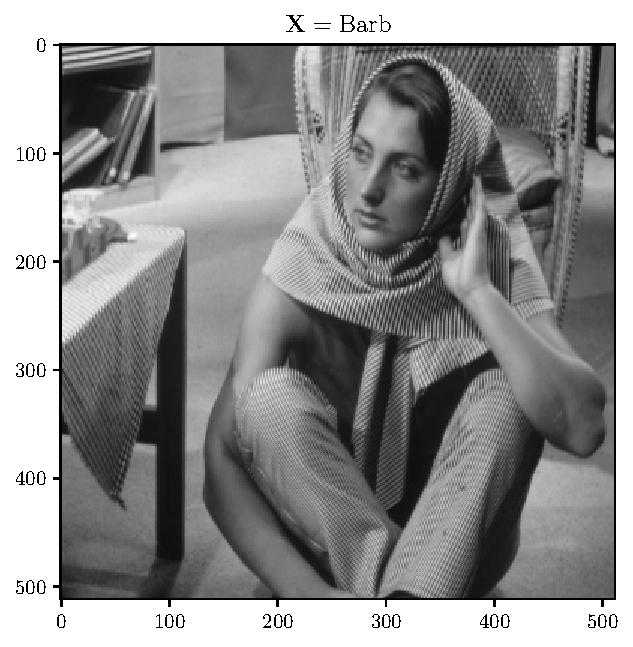
\includegraphics{barb}} & \href{https://nbviewer.org/github/vicente-gonzalez-ruiz/denoising/blob/main/figs/averaging_denoising.ipynb\#0MMGN_barb}{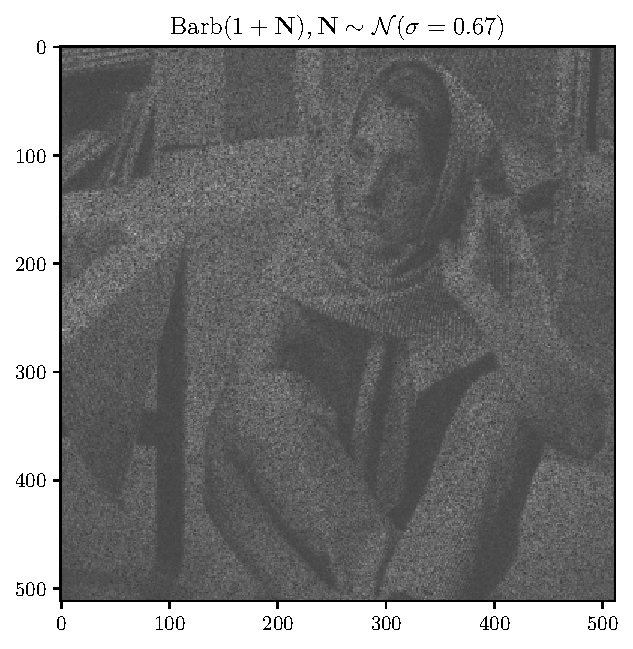
\includegraphics{0MMGN_barb}} \\
        \href{https://nbviewer.org/github/vicente-gonzalez-ruiz/denoising/blob/main/figs/averaging_denoising.ipynb\#denoised_0MMGN_barb}{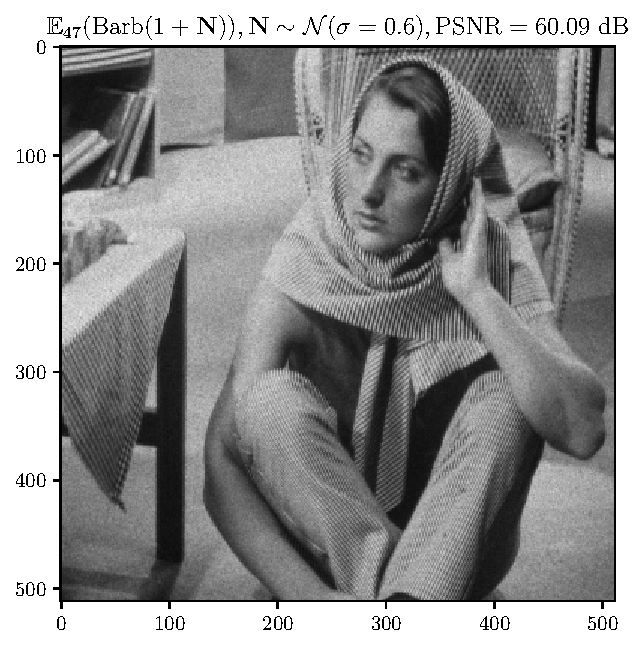
\includegraphics{denoised_0MMGN_barb}} & \href{https://nbviewer.org/github/vicente-gonzalez-ruiz/denoising/blob/main/figs/averaging_denoising.ipynb\#PSNR_0MMGN_barb}{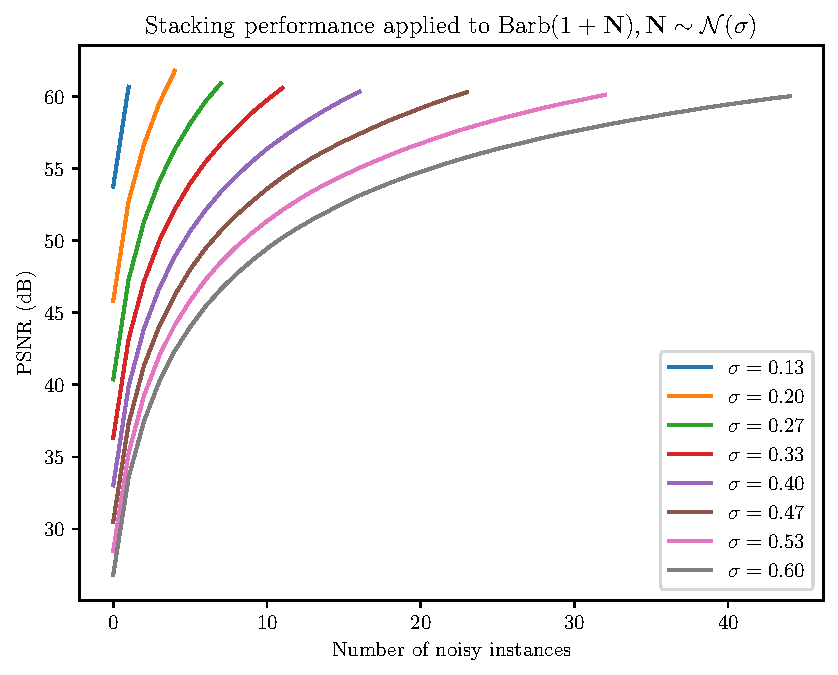
\includegraphics{PSNR_0MMGN_barb}}
      \end{tabular}
    }
    \caption{Effect of zero-mean multiplicative Gaussian noise in an
      image and how averaging can be used to reduced by averaging. The
      clean image of Barb is shown on the top left, and a noisy
      version on the top right. On to bottom, the left image shows a
      denoised version after averaging and the right graph shows the
      performance of the averaging process for different levels of
      noise.\label{fig:0MMGN}}
  \end{figure}

 Fig.~\ref{fig:Rayleigh}
  shows an example of how Rayleigh noise is cancelled by averaging.

  \begin{figure}
    \centering
    \resizebox{1.0\textwidth}{!}{
      \renewcommand{\arraystretch}{0.0} % Adjust row spacing in the table
      \setlength{\tabcolsep}{0ex}      % Adjust column spacing in the table    
      \begin{tabular}{cc}
        \href{https://nbviewer.org/github/vicente-gonzalez-ruiz/denoising/blob/main/figs/averaging_denoising.ipynb\#barb}{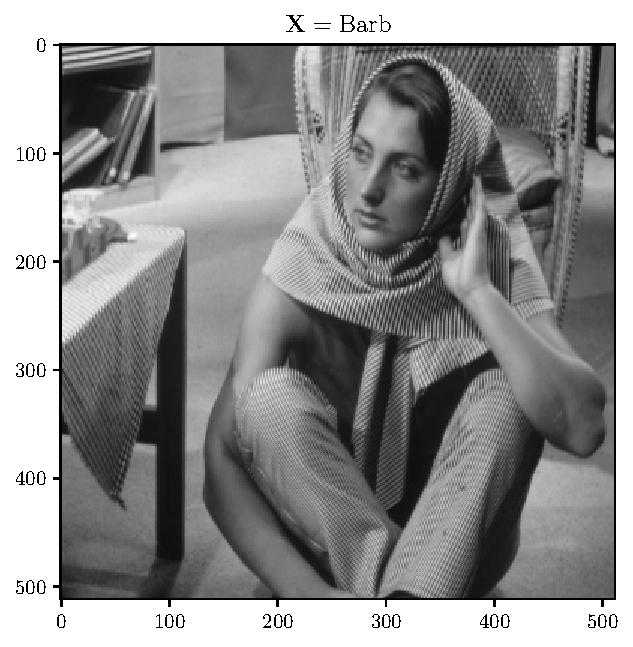
\includegraphics{barb}} & \href{https://nbviewer.org/github/vicente-gonzalez-ruiz/denoising/blob/main/figs/averaging_denoising.ipynb\#Rayleigh_barb}{\includegraphics{Rayleigh_barb}} \\
        \href{https://nbviewer.org/github/vicente-gonzalez-ruiz/denoising/blob/main/figs/averaging_denoising.ipynb\#denoised_Rayleigh_barb}{\includegraphics{denoised_Rayleigh_barb}} & \href{https://nbviewer.org/github/vicente-gonzalez-ruiz/denoising/blob/main/figs/averaging_denoising.ipynb\#PSNR_Rayleigh_barb}{\includegraphics{PSNR_Rayleigh_barb}}
      \end{tabular}
    }
    \caption{Effect of Rayleigh noise in an image and how averaging can
      be used to reduced by averaging. The clean image of Barb is shown
      on the top left, and a noisy version on the top right. On to
      bottom, the left image shows a denoised version after averaging
      and the right graph shows the performance of the averaging
      process for different levels of noise.\label{fig:Rayleigh}}
  \end{figure}

  Fig.~\ref{fig:Poisson} shows an example of how Poisson noise is
  cancelled by averaging.

  \begin{figure}
    \centering
    \resizebox{1.0\textwidth}{!}{
      \renewcommand{\arraystretch}{0.0} % Adjust row spacing in the table
      \setlength{\tabcolsep}{0ex}      % Adjust column spacing in the table    
      \begin{tabular}{cc}
        \href{https://nbviewer.org/github/vicente-gonzalez-ruiz/denoising/blob/main/figs/averaging_denoising.ipynb\#barb}{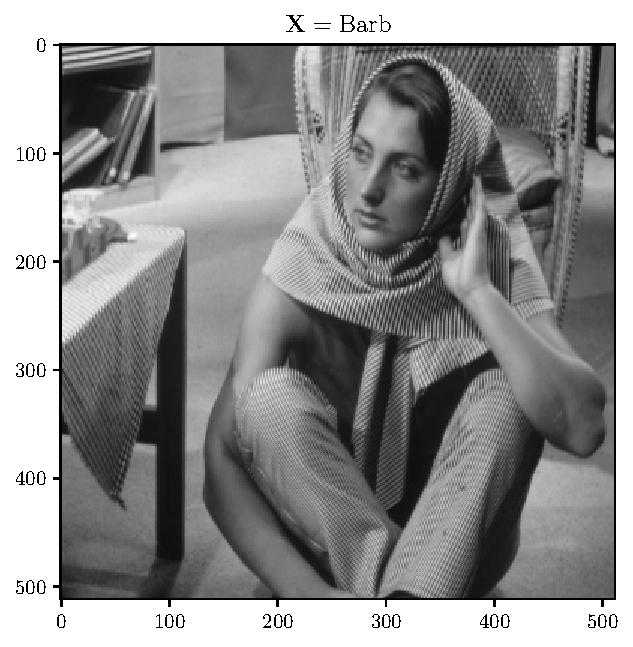
\includegraphics{barb}} & \href{https://nbviewer.org/github/vicente-gonzalez-ruiz/denoising/blob/main/figs/averaging_denoising.ipynb\#Poisson_barb}{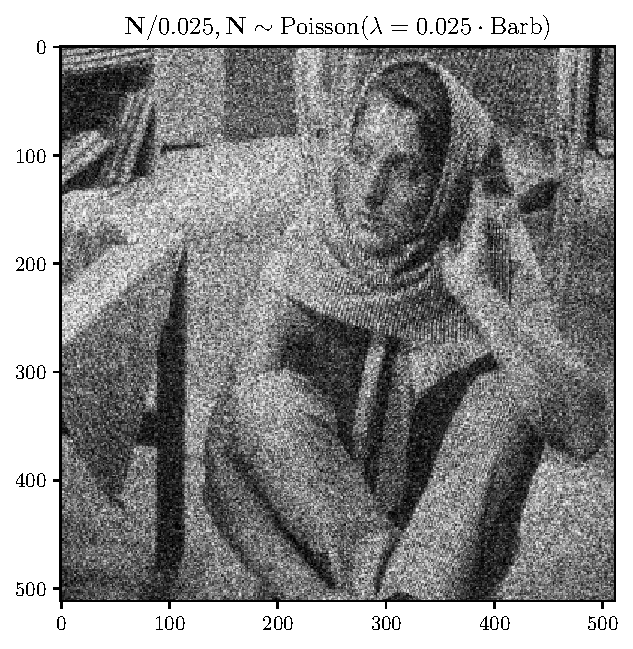
\includegraphics{Poisson_barb}} \\
        \href{https://nbviewer.org/github/vicente-gonzalez-ruiz/denoising/blob/main/figs/averaging_denoising.ipynb\#denoised_Poisson_barb}{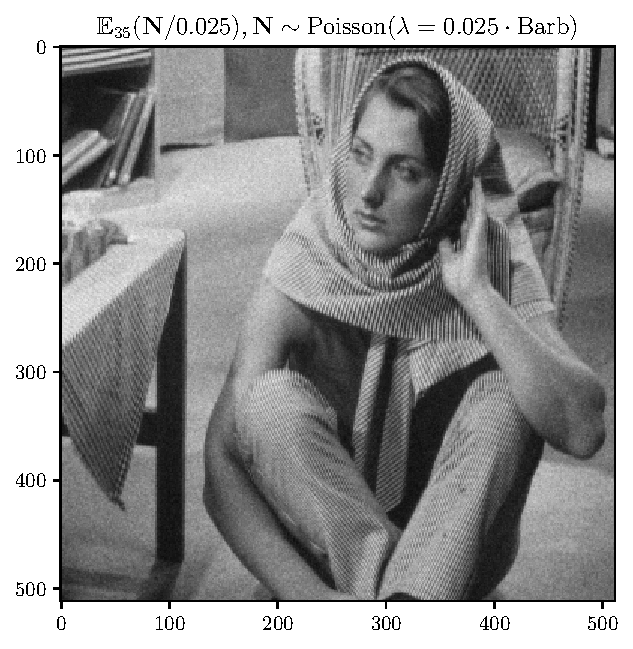
\includegraphics{denoised_Poisson_barb}} & \href{https://nbviewer.org/github/vicente-gonzalez-ruiz/denoising/blob/main/figs/averaging_denoising.ipynb\#PSNR_Poisson_barb}{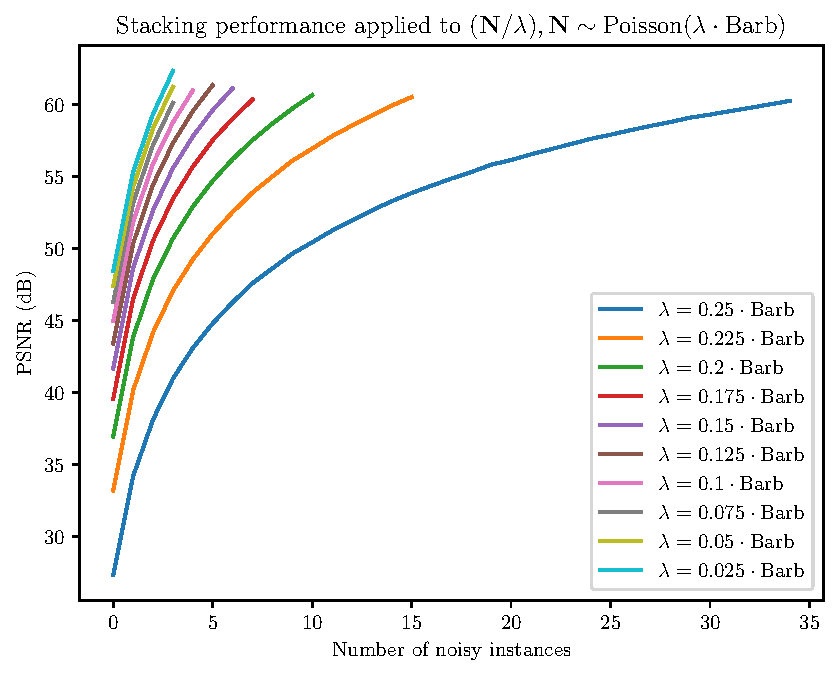
\includegraphics{PSNR_Poisson_barb}}
      \end{tabular}
    }
    \caption{Effect of Poisson noise in an image and how averaging can
      be used to reduced by averaging. The clean image is shown
      on the top left, and a noisy version on the top right. On the
      bottom, the left image shows a denoised version after averaging
      and the right graph shows the performance of the averaging
      process for different levels of noise.\label{fig:Poisson}}
  \end{figure}

%}}}
\end{comment}

%}}}

%}}}
